% myelin water fraction imaging
\begin{frame}{Background}
	\begin{minipage}{0.6\textwidth}
		\uncover<2-3>{%
			Myelin water fraction (MWF): 
  		\begin{itemize}
  			\item<2->{%
  				Proportion of MR signal arising 
  				from water trapped within healthy myelin bilayers,
  				relative to total \hfill \citec{mackay:94:ivv}
  			}
  			\item<3->{%
  				Correlates well with myelin content \hfill \citec{webb:03:imt}
  			}
  		\end{itemize}
		}
	\end{minipage}
	\begin{minipage}{0.36\textwidth}
		\uncover<1-3>{%
			\begin{figure}
				\centering
				\includegraphics[width=3.5cm]{c,mwf/myelin}
			\end{figure}
			\hfill www.mayoclinic.org
		}
	\end{minipage}
\end{frame}

\begin{frame}{Previous MWF imaging acquisitions}
	\uncover<1>{%
  	Multi-echo spin-echo (\textbf{MESE}) \hfill \citec{mackay:94:ivv}
  	\begin{itemize}
  		\item{Gold-standard}
  		\item{Speed-limited by long repetition times ($\sim$2s)}
  	\end{itemize}
  }
  \uncover<2>{%
  	Combinations of fast steady-state scans using variable flip angles (``\textbf{mcDESPOT}'') 
  		\hfill \citec{deoni:08:gmt}
  	\begin{itemize}
  		\item{Whole-brain, high-resolution MWF imaging in $\sim$30m}
  		\item{%
  			Disagree with MESE MWF estimates, \hfill \citec{zhang:15:com}
  			likely due to insufficient precision \hfill \citec{lankford:13:oti}
  		}
  	\end{itemize}
	}
	\uncover<3->{%
		\textbf{Goal}: fast, precise MWF quantification in WM
	}
\end{frame}

\begin{frame}{A voxel-scale MWF model}
	\begin{figure}
		\begin{tikzpicture}
			\uncover<1->{
				\node[above] at (2,4) {simple two-compartment model};
				\draw[thick,fill=gray!10] (0,0) -- (2,0) -- (1,4) -- (0,4) -- (0,0);
				\draw[thick,fill=gray!30] (2,0) -- (4,0) -- (4,4) -- (1,4);
				\node[below] at (1,0) {``fast''};
				\node[below] at (3,0) {``slow''};
			}
			\only<2-3>{
				\node[below right] at (0,0.7) {$\tf{1},\tf{2}$};
				\node[below left] at (4,0.7) {$\ts{1},\ts{2}$};
  			\alt<2>{
  				\node at (2.7,2) {$\paren{1-\ff}\mzero$};
  				\node at (0.7,2) {$\ff \mzero$};
  			}{
  				\node at (2.7,2) {$\paren{1-\hlg{\ff}}\mzero$};
  				\node at (0.7,2) {$\hlg{\ff} \mzero$};
  			}
			}
		\end{tikzpicture}
	\end{figure}
	\uncover<3->{
		Take fast-relaxing fraction $\hlg{\ff}$ as a simple proxy for MWF
	}
\end{frame}

\begin{frame}{Multi-compartmental MR signal models}
	\uncover<1-3>{%
		2-compartment SPGR model \hfill \citec{spencer:00:mos} \\
	}
	\begin{itemize}
		\item<1>{included first-order physical exchange}
		\item<2,5>{neglected relaxation, precession, exchange during excitation}
		\item<3,5>{%
			absorbing off-resonance effects into $\mzero$ 
			\emph{implies} neglecting exchange between excitation and readout
		}
	\end{itemize}
	\uncover<4->{%
		Two-compartment DESS model \hfill \textcolor{arch-ivy}{\S6.2.2}%
	}
	\begin{itemize}
		\item<4-5>{%
			additional approximations required 
			unless we assume time-independent diff 
			in compartmental off-resonance freq
		}
		\item<5>{%
			including exchange, closed-form solutions still elusive
		}
	\end{itemize}
	\uncover<6>{%
		\textbf{For simplicity, we neglect exchange.}
	}
\end{frame}

\begin{frame}{Bayesian MWF Scan Design}
	\begin{align}
    \breve{\bmP} &\in 
    	\set{
        \argmin{\bmP \in \setP}
        \expcost\paren{\bmP}
    	}, \where \nonumber \\
		\expcost\paren{\bmP} &:=
    	\expect{\bmx,\bmnu}{\trace{\bmW \bmF^{-1}\paren{\bmx; \bmnu, \bmP} \bmW\tpose}}
  \end{align}
  \vspace{-0.5cm}
  \begin{itemize}
  	\item<2>{%
			\makebox[1.5cm][l]{$\bmx$} 
			$\brac{\hlg{\ff}, \tf{1}, \tf{2}, \ts{1}, \ts{2}, \mzero}\tpose$
		}
		\item<2>{%
			\makebox[1.5cm][l]{$\bmnu$}
			flip angle variation
		}
		\item<2>{%
			\makebox[1.5cm][l]{$\bmP$}
			SPGR/DESS nominal flip angles, repetition times
		}
		\item<3>{%
			\makebox[1.5cm][l]{$\bmW$}
			$\diag{\brac{\inv{\expect{\bmx,\bmnu}{\hlg{\ff}}}, \zeros{5}\tpose}\tpose}$
		}
		\item<4>{%
			\makebox[1.5cm][l]{$\expect{\bmx,\bmnu}{\cdot}$}
			approximated via empirical averages \\
			\makebox[1.5cm][l]{}
			of samples drawn from separable prior
		}
		\item<5>{%
			\makebox[1.5cm][l]{$\setP$}
			nom flip angle, total scan time constraints
		}
  \end{itemize}
\end{frame}

\begin{frame}{Optimized SPGR/DESS Acquisition}
	\begin{table}[!tb]
    \centering
    \begin{tabular}{r | c | c}
      \hline
      \hline
      & Optimized flip angles (deg) & Optimized rep. times (ms) \\
      \hline
      SPGR & $38.1,12.9,9.2,33.5$ 	& $50.2,32.4,16.4,11.8$ \\
      DESS & $32.0,40.3,52.9$ 			& $17.5,98.0,37.6$ \\
      \hline
      \hline
    \end{tabular}
    \caption{Optimized Scan Parameters, $\breve{\bmP}$}
		\label{tab:mwf,acq}
	\end{table}
	\begin{itemize}
		\item{%
			Predicted MWF relative standard deviation in WM
			\begin{itemize} 
				\item{%
					Optimized SPGR/DESS:
					$\sqrt{\expcost\paren{\breve{\bmP}}} = 0.285$
				}
				\item{%
					mcDESPOT: at least $1$ \hfill \citec{lankford:13:oti}
				}
			\end{itemize}
		} 
	\end{itemize}
\end{frame}

\begin{frame}{MWF Estimation via KRR}
	\uncover<1>{%
		\textbf{Simulation Setup}
		\begin{itemize}
			\item{At each voxel, generate ground-truth $\bmx,\bmnu$}
			\item{Using 2-compartment SPGR/DESS model $\bms$
				with optimized (and now fixed) parameters $\breve{\bmP}$,
				generate voxel data $\bmy \in \complexes{10}$
			}
		\end{itemize}
	}
	\uncover<2>{%
		\textbf{Use KRR to estimate just $\hlg{\ff}$}
		\begin{itemize}
			\item{Separable prior on $\bmx$: $\hlg{\ff},\mzero$ uniform; others log-uniform}
			\item{$N \gets 10^6$ training points}
			\item{$Z \gets 10^3$ kernel approximation order}
		\end{itemize}
	}
	\uncover<3>{%
		\textbf{Compare against grid search}
		\begin{itemize}
			\item{unconstrained search would require $\sim$100$^{5}$ dictionary atoms}
			\item{we artificially constrain search here to limit computation}
		\end{itemize}
	}
\end{frame}

\begin{frame}{MWF Simulation Result}
	Fast-fraction $\hlg{\ff}$ estimates, in simulation: 
	\uncover<+->{%
		\begin{figure}[t]
			\centering
			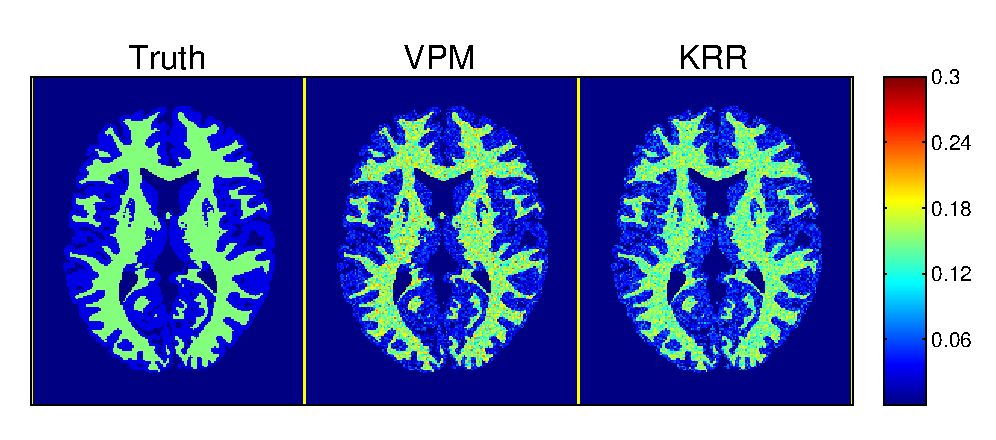
\includegraphics[width=\textwidth]{c,krr/sim}%
		\end{figure}
	}
	\uncover<+->{%
		\makebox[5cm][r]{$\sim$4h}
		\makebox[4.7cm][r]{$40$s training, $2$s testing}
	}	
\end{frame}

\begin{frame}{MWF Proof-of-concept Experimental Study}
	\uncover<1>{%
		Acquired \invivo data using optimized MWF protocol
		\begin{itemize}
			\item{Used $256\times256\times8$ 3D matrix over $24\times24\times4$cm FOV}
			\item{Required \textbf{11m48s} total (including BS scan)} 
		\end{itemize} 
	}
	\uncover<2-4>{%
		Rapidly estimated $\hlg{\ff}$ as proxy for MWF
		\begin{itemize}
			\item<2>{Full-scale grid search intractable on typical desktop}
			\item<3-4>{KRR training and testing took \textbf{35s} and \textbf{5s/slice}}
			\item<4>{Iterative ML refinement took \textbf{29s/slice}}
		\end{itemize}
	}
	\uncover<5->{%
		Compared (qualitatively) with results in \hfill \citec{zhang:15:com}%
		\begin{itemize}
			\item{GRASE: accelerated MESE acq \hfill \citec{prasloski:12:rwc}}
			\item{mcDESPOT: 9 SPGR, 18 bSSFP scans \hfill \citec{deoni:11:com}}
		\end{itemize}	
	}
\end{frame}

\begin{frame}{MWF Proof-of-concept In Vivo Result}
	\vspace{-0.3cm}
	\begin{figure}
    \centering
    \begin{minipage}[b]{0.7\textwidth}
        \centering
        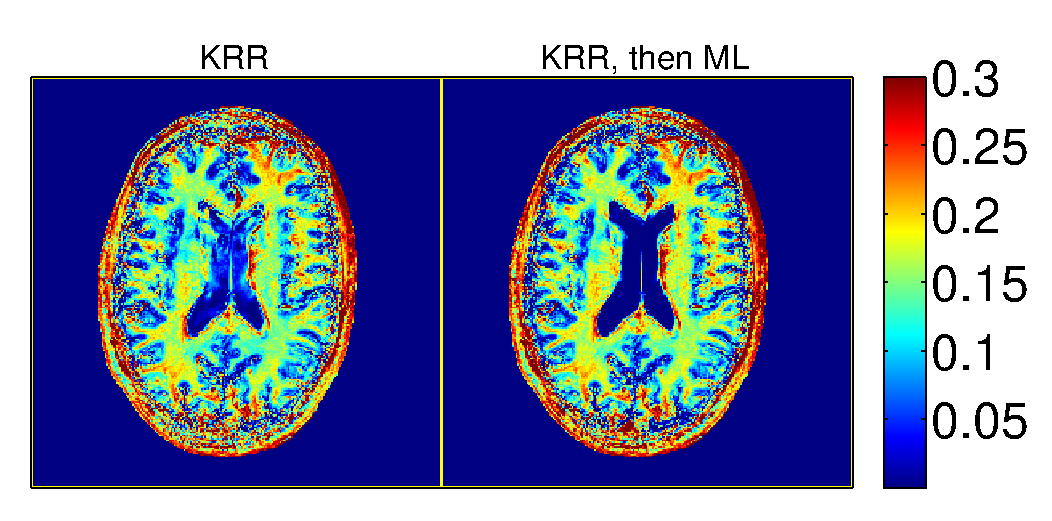
\includegraphics [height=4cm, clip] {c,mwf/ff,log2c-0,krr-ml}
    \end{minipage}

    \begin{minipage}[b]{0.96\textwidth}
        \centering
        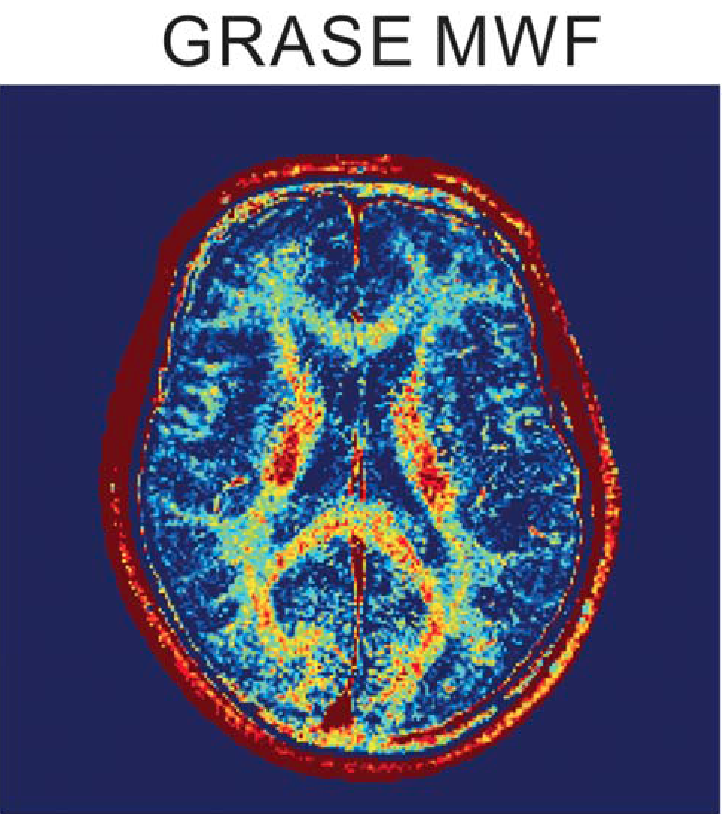
\includegraphics [height=3.8cm] {c,mwf/mwf,grase}
        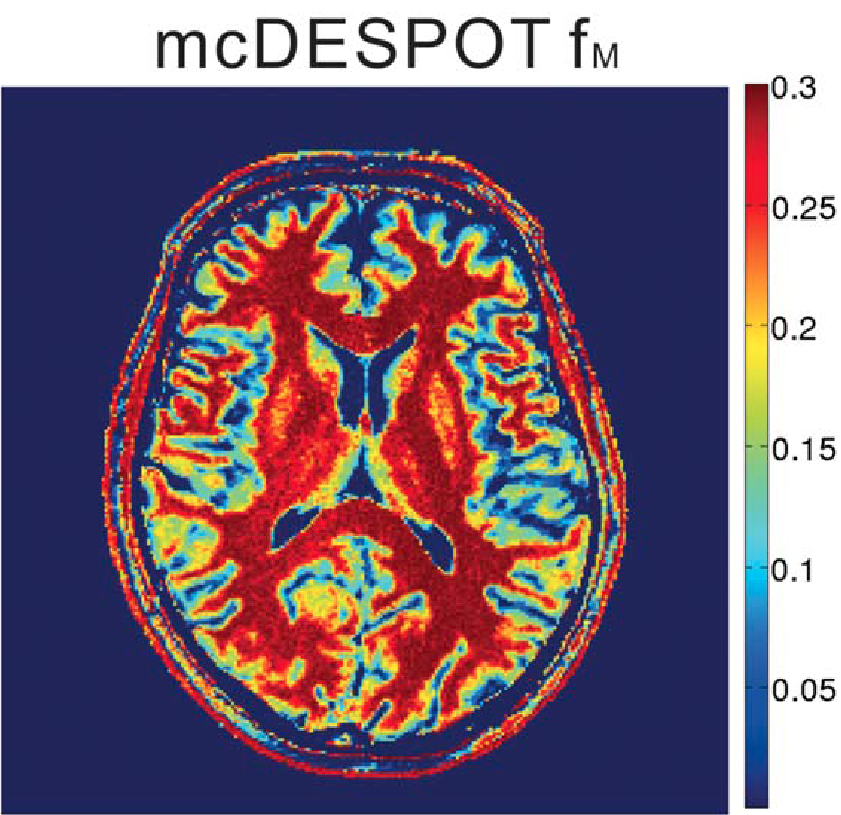
\includegraphics [height=3.8cm] {c,mwf/mwf,mcdespot}
    \end{minipage}
 	\end{figure}
\end{frame}

\begin{frame}{Summary}
	\uncover<1->{%
  	\textbf{Contributions}
  	\begin{itemize}
  		\item{Two-compartment DESS signal model}
  		\item{Fast acquisition for precise WM MWF estimation}
			\item{Proof-of-concept \invivo MWF images via KRR}
  	\end{itemize}
	}
	\uncover<2->{%
  	\textbf{Ongoing work}
  	\begin{itemize}
  		\item<2>{Systematic validation}
  		\item<3>{Further-optimized MWF acquisition}
  	\end{itemize}
	}
\end{frame}
